\RequirePackage{plautopatch}
\documentclass[uplatex, a4paper, 14Q, dvipdfmx]{jsarticle}
\usepackage{docmute}
\usepackage{../mypackage}

\title{安定\texorpdfstring{$\infty$}{infty}圏}
\author{よの}
\date{\today}

\begin{document}

\maketitle

\begin{abstract}
\end{abstract}

\tableofcontents

\section{安定\texorpdfstring{$\infty$}{infty}圏}

\begin{definition}[基点付き$\infty$圏]
  $\C$を$\infty$圏とする.
  $\C$の対象$0$が始対象かつ終対象であるとき, $0$を零対象(zero object)という.
  $\C$が零対象を持つとき, $\C$は基点付き(pointed)であるという.
\end{definition}

\begin{lemma}
  $\C$を$\infty$圏, $0$を$\C$の対象とする.
  このとき, 次の2つは同値である. 
  \begin{enumerate}
    \item $0$は零対象である. 
    \item 任意の$X \in \C$に対して, $\Map_\C(X,0)$と$\Map_\C(0,X)$は可縮である. 
  \end{enumerate}
\end{lemma}

\begin{remark}
  零対象は存在すれば同値を除いて一意である. 
\end{remark}

\begin{definition}[簡約関手]
  $\C,\D$を基点付き$\infty$圏, $\F : \C \to \D$を$\infty$圏の関手とする. 
  $\F$が零対象を保つとき, $\F$は簡約(reduced)であるという.
  簡約関手のなす$\fun(\C,\D)$の部分圏を$\fun_\ast(\C,\D)$と表す. 
\end{definition}

\begin{definition}[ヌルホモトピー]
  $\C$を基点付き$\infty$圏, $f : X \to Y$を$\C$の射とする.
  次の図式で表される$2$単体$\Delta^2 \to \C$を$f$のヌルホモトピーという.
  また, ヌルホモトピーを持つ$f$を$0$射($0$-map)という. 
  \[
    \begin{tikzpicture}[auto,->]
      \node (0) at (1,0) {$0$};
      \node (X) at (0,1) {$X$};
      \node (Y) at (2,1) {$Y$};
      \draw (X) -- node {$f$} (Y);
      \draw (X) -- (0);
      \draw (0) -- (Y);
    \end{tikzpicture}
  \]
\end{definition}

\begin{lemma}
  $\C$を$\infty$圏とする.
  $\C$が基点付きであることと, 次の3つの条件を満たすことは同値である. 
  \begin{enumerate}
    \item $\C$は始対象$\emptyset$を持つ.
    \item $\C$は終対象$1$を持つ. 
    \item $\C$の射$f : 1 \to \emptyset$が存在する. 
  \end{enumerate}
\end{lemma}

\begin{proof}
  $\C$が基点付きであるとき, 3つの条件を満たすことは明らかである. \\
  逆に, 条件(1)から(3)が満たされているとする.
  $\emptyset$は始対象なので, 射$g : \emptyset \to 1$が存在する.
  $\emptyset$は始対象なので, $fg \simeq \id_\emptyset$である.
  $1$は終対象なので, $gf \simeq \id_1$である. 
  よって, $g$は$f$のホモトピー逆射なので, $f$は同型射である.
  従って, $\emptyset$は終対象でもあるので, $\C$は基点付きである. 
\end{proof}

\begin{definition}[(コ)ファイバー]
  $\C$を基点付き$\infty$圏とする.
  次の形で表される射$\Delta^1 \times \Delta^1 \to \C$を$\C$の三角(diagram)という. 
  \[
    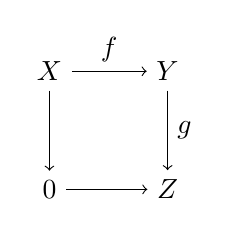
\begin{tikzpicture}[auto,->]
      \node (0) at (0,0) {$0$};
      \node (Z) at (1.5,0) {$Z$};
      \node (X) at (0,1.5) {$X$};
      \node (Y) at (1.5,1.5) {$Y$};
      \draw (0) -- (Z);
      \draw (X) -- (0);
      \draw (X) -- node{$f$} (Y);
      \draw (Y) -- node{$g$} (Z);
    \end{tikzpicture}
  \]
  この三角がpullbackであるとき, 三角をファイバー列(fibre sequence)という.
  双対的に, この三角がpushoutであるとき, 三角をコファイバー列(cofibre sequence)という.

  このようなファイバー列が存在するとき, $g$はファイバーを持つという. 
  双対的に, このようなコファイバー列が存在するとき, $f$はコファイバーを持つという. 
  このとき, $X:=\fib{g}, Z := \cofib{f}$と表す. 

  また, $\C$の任意の射が(コ)ファイバーを持つとき, $\C$は(コ)ファイバーを持つという. 
\end{definition}

\begin{remark}
  $\C$を基点付き$\infty$圏とする.
  $\C$の三角は次のデータから構成される.
  \begin{enumerate}
    \item $\C$の射$f : X \to Y$と$g : Y \to Z$
    \item $h$が$g$と$f$の合成であることを表す$2$単体
    \[
      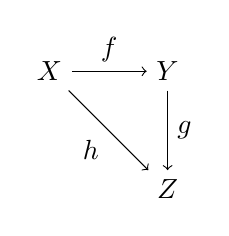
\begin{tikzpicture}[auto,->]
        \node (Z) at (1.5,0) {$Z$};
        \node (X) at (0,1.5) {$X$};
        \node (Y) at (1.5,1.5) {$Y$};
        \draw (X) -- node{$f$} (Y);
        \draw (Y) -- node{$g$} (Z);
        \draw (X) -- node[swap]{$h$} (Z);
      \end{tikzpicture}
    \]
    \item $h$のヌルトピックを表す$2$単体
    \[
      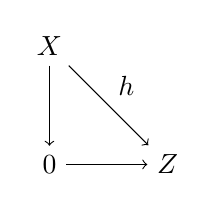
\begin{tikzpicture}[auto,->]
        \node (0) at (0,0) {$0$};
        \node (Z) at (1.5,0) {$Z$};
        \node (X) at (0,1.5) {$X$};
        \draw (0) -- (Z);
        \draw (X) -- (0);
        \draw (X) -- node{$h$} (Z);
      \end{tikzpicture}
    \]
  \end{enumerate} 
\end{remark}

\begin{notation}
  $\C$を基点付き$\infty$圏とする.
  $\C$の三角を
  \begin{align*}
    X \xrightarrow{f} Y \xrightarrow{g} Z
  \end{align*}
  と表す. 
\end{notation}

\begin{definition}[安定$\infty$圏]
  基点付き$\infty$圏$\C$が次の条件を満たすとき, $\C$は安定(stable)であるという. 
  \begin{enumerate}
    \item $\C$はファイバーとコファイバーを持つ.
    \item $\C$の三角がファイバー列であることとコファイバー列であることは同値である.
  \end{enumerate}
\end{definition}

\begin{remark}
  安定$\infty$圏は$\infty$圏に追加の構造を持たせたものではなく, $\infty$圏の持つ性質を用いて定義されている. 
\end{remark}

\begin{lemma} \label{prop:Cop_is_also_stable}
  $\C$が安定$\infty$圏であるとき, $\C^\myop$も安定$\infty$圏である.
\end{lemma}

\begin{proof}
  安定$\infty$圏の定義が双対的であることから従う. 
\end{proof}

\begin{definition}[完全関手]
  $\C,\D$を安定$\infty$圏, $\F : \C \to \D$を$\infty$圏の関手とする.
  $\F$が$0$対象とファイバー列, コファイバー列を保つとき, $\F$は完全(exact)であるという.
  完全関手のなす$\fun_\ast(\C,\D)$の部分圏を$\fun^\ex(\C,\D)$と表す. 
\end{definition}


\section{安定\texorpdfstring{$\infty$}{infty}圏のホモトピー圏}

$\C$を基点付き$\infty$圏, $0$と$0'$を$\C$の零対象とする. 
次のpushoutで表される図式の$\fun(\Delta^1 \times \Delta^1,\C)$の充満部分圏を$\M^\Sigma$と表す. 
\[
  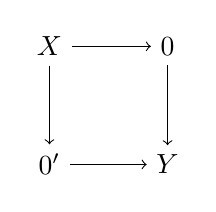
\begin{tikzpicture}[auto,->]
    \node (0') at (0,0) {$0'$};
    \node (Y) at (1.5,0) {$Y$};
    \node (X) at (0,1.5) {$X$};
    \node (0) at (1.5,1.5) {$0$};
    \draw (X) -- (0);
    \draw (X) -- (0');
    \draw (0') -- (Y);
    \draw (0) -- (Y);
  \end{tikzpicture}
\]
HTT.4.3.2.15を2回用いると, 自明なファイブレーション$e : \M^\Sigma \to \C$を得る. 
$s : \C \to \M^\Sigma$を$e$の切断とする.
このとき, 
\begin{align*}
  \Sigma_\C := e \circ s : \C \to \C
\end{align*}
を$\C$上の懸垂(suspention functor)という. 
双対的に, 同じ形のpulbackで表される$\fun(\Delta^1 \times \Delta^1,\C)$の充満部分圏を$\M^\Omega$と表す. 
$\C$がファイバーを持つとき, 同様に自明なファイブレーション$e' : \M^\Omega \to \C$を得る. 
$s' : \C \to \M^\Omega$を$e'$の切断とする.
このとき, 
\begin{align*}
  \Omega\C := e' \circ s' : \C \to \C
\end{align*}
を$\C$上のループ(loop functor)という. 
$\C$が安定であるとき, $\M^\Sigma = \M^\Omega$である. 

\begin{notation}
  $\C$を安定$\infty$圏とする.
  任意の$X \in \C$と$n \geq 0$に対して, 
  \begin{align*}
    X[n] := \Sigma^n(X)
  \end{align*}
  と表し, 懸垂の$n$乗($n$-th power)という. 
  $n \leq 0$に対して, 
  \begin{align*}
    X[n] := \Omega^n(X) 
  \end{align*}
  と表し, ループの$-n$乗という. 
  誘導されるホモトピー圏上の関手の対応も同じ記号を用いて表す.
\end{notation}

\begin{remark}
  $\C$が基点付き$\infty$圏のとき, 懸垂とループはホモトピー逆射ではないが, 随伴ではある.
\end{remark}


\section{安定\texorpdfstring{$\infty$}{infty}圏における(余)極限}

安定$\infty$圏の定義にはファイバーとコファイバーのみを用いて定義されたが, 任意の有限極限と有限余極限を持つことが分かる. 

\begin{lemma} \label{prop:stable_has_pushout_pullback}
  $\C$を安定$\infty$圏とする.
  このとき, 次の2つが従う.
  \begin{enumerate}
    \item $\C$はpushoutとpullbackを持つ. 
    \item $\C$における四角がpushoutであることとpullbackであることは同値である.
  \end{enumerate}
\end{lemma}

\begin{proof}
  (1)を示す.
  \cref{prop:Cop_is_also_stable}より, $\C$がpushoutを持つことを示せばよい.
  次の図式を考える.
  \[
    \begin{tikzpicture}[auto,->]
      \node (Y) at (0,0) {$Y$};
      \node (W) at (0,1.5) {$W$};
      \node (X) at (1.5,1.5) {$X$};
      \draw (W) -- node {$g$} (X);
      \draw (W) -- node {$f$} (Y);
    \end{tikzpicture}
  \]
  $f$がファイバーを持つので, 次の図式が存在する.
  \[
    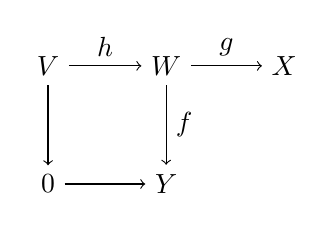
\begin{tikzpicture}[auto,->]
      \node (V) at (-1.5,1.5) {$V$};
      \node (0) at (-1.5,0) {$0$};
      \node (Y) at (0,0) {$Y$};
      \node (W) at (0,1.5) {$W$};
      \node (X) at (1.5,1.5) {$X$};
      \draw (V) -- node {$h$} (W);
      \draw (V) -- (0);
      \draw (0) -- (Y);
      \draw (W) -- node {$g$} (X);
      \draw (W) -- node {$f$} (Y);
    \end{tikzpicture}
  \]
  ここで, 左の四角はファイバー列である.
  合成$gh$はコファイバーを持ち, 左の四角はコファイバー列でもであるので 次の図式が存在する.
  \[
    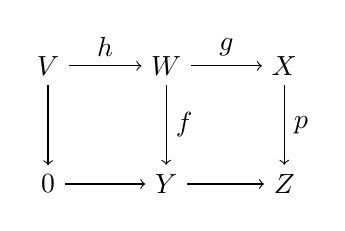
\begin{tikzpicture}[auto,->]
      \node (V) at (-1.5,1.5) {$V$};
      \node (0) at (-1.5,0) {$0$};
      \node (Y) at (0,0) {$Y$};
      \node (W) at (0,1.5) {$W$};
      \node (X) at (1.5,1.5) {$X$};
      \node (Z) at (1.5,0) {$Z$};
      \draw (V) -- node {$h$} (W);
      \draw (V) -- (0);
      \draw (0) -- (Y);
      \draw (W) -- node {$g$} (X);
      \draw (W) -- node {$f$} (Y);
      \draw (X) -- node {$p$} (Z);
      \draw (Y) -- (Z);
    \end{tikzpicture}
  \]
  ここで, 外側の四角はpushoutである. 
  左と外側の四角はpushoutなので, 右側の四角もpushoutである. 

  (2)を示す.
  \cref{prop:Cop_is_also_stable}より, 任意のpullbackがpushoutであることを示せばよい.
  次のpulbackを考える. 
  \[
    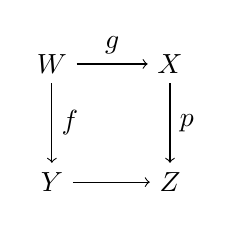
\begin{tikzpicture}[auto,->]
      \node (Y) at (0,0) {$Y$};
      \node (W) at (0,1.5) {$W$};
      \node (X) at (1.5,1.5) {$X$};
      \node (Z) at (1.5,0) {$Z$};
      \draw (W) -- node {$g$} (X);
      \draw (W) -- node {$f$} (Y);
      \draw (X) -- node {$p$} (Z);
      \draw (Y) -- (Z);
    \end{tikzpicture}
  \]
  (1)と同様に, $f$がファイバーを持つので, 次の図式が存在する.
  \[
    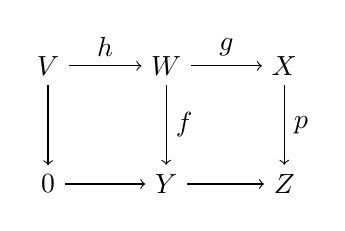
\begin{tikzpicture}[auto,->]
      \node (V) at (-1.5,1.5) {$V$};
      \node (0) at (-1.5,0) {$0$};
      \node (Y) at (0,0) {$Y$};
      \node (W) at (0,1.5) {$W$};
      \node (X) at (1.5,1.5) {$X$};
      \node (Z) at (1.5,0) {$Z$};
      \draw (V) -- node {$h$} (W);
      \draw (V) -- (0);
      \draw (0) -- (Y);
      \draw (W) -- node {$g$} (X);
      \draw (W) -- node {$f$} (Y);
      \draw (X) -- node {$p$} (Z);
      \draw (Y) -- (Z);
    \end{tikzpicture}
  \]
  左の四角はファイバー列かつコファイバー列なので, 外側の四角はpullbackかつpushoutである.
  (1)より, 右の四角はpushoutでもある.
\end{proof}

\begin{lemma}
  $\F : \C \to \D$を安定$\infty$圏の関手とする. 
  このとき, 次の2つは同値である.
  \begin{enumerate}
    \item $\F$は完全である.
    \item $\F$は零対象とpushoutを保つ.
    \item $\F$は零対象とpullbackを保つ.
  \end{enumerate}
\end{lemma}

\begin{proof}
  (2)と(3)の同値性は\cref{prop:stable_has_pushout_pullback}の(2)より従う.\\
  (1)と(2)の同値性は完全関手がpushoutを保つことを示せばよい. 
  これは\cref{prop:stable_has_pushout_pullback}の(1)と同様の議論で示せる.
\end{proof}

\begin{theorem}
  $\C$を安定$\infty$圏, $\F : \C \to \D$を安定$\infty$圏の関手とする.
  このとき, 次の2つが従う. 
  \begin{enumerate}
    \item $\C$は任意の有限極限と有限余極限を持つ.
    \item $\F$が完全であることと, $\F$が有限(余)極限を保つことは同値である. 
  \end{enumerate}
\end{theorem}

\begin{prop}
  $\C$を基点付き$\infty$圏とする.
  このとき, 次の3つは同値である.
  \begin{enumerate}
    \item $\C$は安定である.
    \item $\C$はコファイバーを持ち, 懸垂関手は$\infty$圏同値である. 
    \item $\C$はファイバーを持ち, ループ関手は$\infty$圏同値である. 
  \end{enumerate}
\end{prop}

\begin{proof}
  \cref{prop:Cop_is_also_stable}より, (2)と(3)の同値性は従う. \\
  (1)から(2)と(1)から(3)はすでに示している.\\
  (2)から(1)を示す.
  $\C$をコファイバーを持つ基点付き$\infty$圏, $\Sigma_\C$は$\infty$圏同値であるとする.
  $\C$が安定であるのは, 次の3つを示せばよい. 
  \begin{enumerate}
    \item $\C$の任意のコファイバー列はファイバー列である. 
    \item $\C$はファイバーを持つ.
    \item $\C$の任意のファイバー列はコファイバー列である. 
  \end{enumerate}
  
\end{proof}


\end{document}